\begin{figure}[htbp]
\section*{EZH1}
\centering
\begin{subfigure}[b]{0.95\textwidth}
\centering
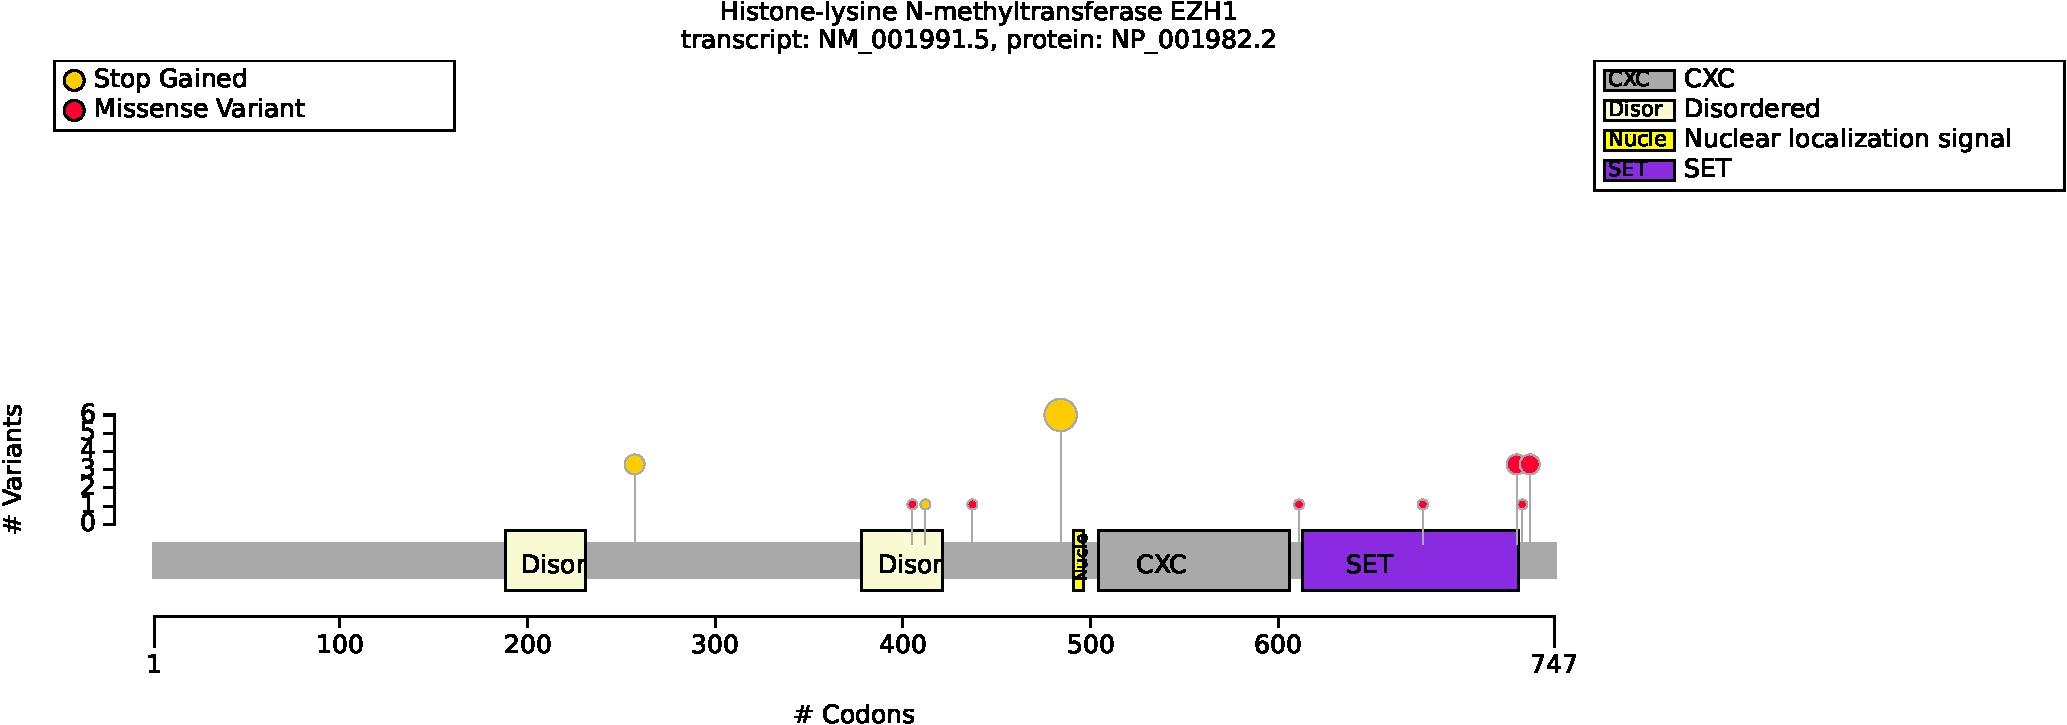
\includegraphics[width=\textwidth]{ img/EZH1_protein_diagram.pdf} 
\captionsetup{justification=raggedright,singlelinecheck=false}
\caption{Distribution of variants in EZH1}
\end{subfigure}

\vspace{2em}

\begin{subfigure}[b]{0.95\textwidth}
\centering
\resizebox{\textwidth}{!}{
\begin{tabular}{llllrr}
\toprule
Genotype (A) & Genotype (B) & total tests performed & significant results\\
\midrule
1 allele & 2 alleles & 33 & 0\\
\bottomrule
\end{tabular}
}
\captionsetup{justification=raggedright,singlelinecheck=false}
\caption{Fisher Exact Test performed to compare HPO annotation frequency with respect to monoallelic and biallelic pathogenic variants. }
\end{subfigure}

\vspace{2em}

\caption{The cohort comprised 19 individuals (10 females, 8 males, 1 with unknown sex). A total of 106 HPO terms were used to annotate the cohort. Disease diagnosis: EZH1-related neurodevelopmental disorder (OMIM:601674). No statistically significant results identified. A total of 12 unique variant alleles were found in \textit{EZH1} (transcript: \texttt{NM\_001991.5}, protein id: \texttt{NP\_001982.2}). In the original publication, it is stated that patients show neurodevelopmental delay with variable clinical presentations regardless of variant type and zygosity \cite{PMID_37433783}.}
\end{figure}
